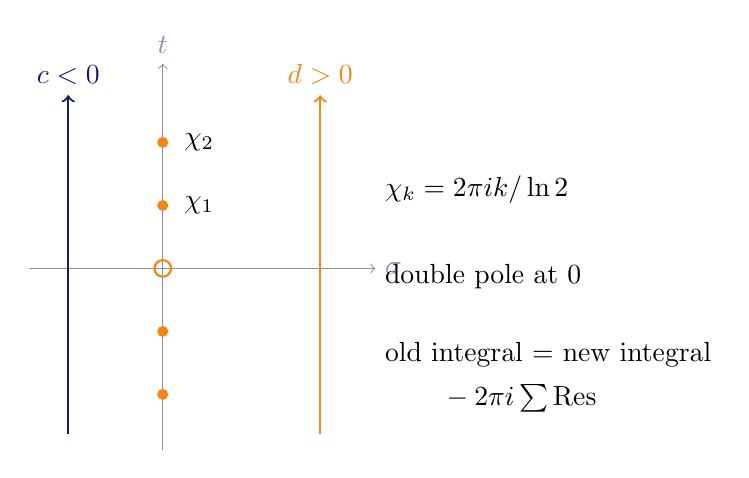
\begin{tikzpicture}[x=1cm,y=1cm]
\draw[->,MidnightBlue!50] (-1.7,0)--(2.7,0) node[right] {$\sigma$};
\draw[->,MidnightBlue!50] (0,-2.3)--(0,2.6) node[above] {$t$};
\draw[thick,MidnightBlue,->] (-1.2,-2.1)--(-1.2,2.2) node[above] {$c<0$};
\draw[thick,BurntOrange,->] (2,-2.1)--(2,2.2) node[above] {$d>0$};
\foreach \y in {-1.6,-.8,.8,1.6}{\fill[BurntOrange] (0,\y) circle (2pt);}
\draw[BurntOrange,thick] (0,0) circle (3pt);
\node[right] at (.15,.8) {$\chi_1$};\node[right] at (.15,1.6) {$\chi_2$};
\node[right] at (2.7,1) {$\chi_k=2\pi ik/\ln2$};
\node[right] at (2.7,-.1) {double pole at $0$};
\node[right] at (2.7,-1.1) {old integral $=$ new integral};
\node[right] at (2.7,-1.65) {$\qquad{}-2\pi i\sum\mathrm{Res}$};
\end{tikzpicture}
